% Generated fragments require trusted human review before compilation.
% This binder never requests shell escape or runs external tools.
\documentclass[11pt]{article}
% Trusted shared apparatus. Requires LuaLaTeX; never use shell escape.
\usepackage{fontspec}
\defaultfontfeatures{Ligatures=TeX}
\IfFontExistsTF{Noto Serif}{\setmainfont{Noto Serif}}{%
  \IfFontExistsTF{DejaVu Serif}{\setmainfont{DejaVu Serif}}{%
    \IfFontExistsTF{Times New Roman}{\setmainfont{Times New Roman}}{%
      \PackageError{gelfand-binder}{No configured Cyrillic serif font installed}{Install Noto Serif or DejaVu Serif, or select an installed Cyrillic font.}%
    }%
  }%
}
\IfFontExistsTF{Noto Sans}{\setsansfont{Noto Sans}}{%
  \IfFontExistsTF{DejaVu Sans}{\setsansfont{DejaVu Sans}}{\setsansfont{Arial}}%
}
\IfFontExistsTF{Noto Sans Mono}{\setmonofont{Noto Sans Mono}}{%
  \IfFontExistsTF{DejaVu Sans Mono}{\setmonofont{DejaVu Sans Mono}}{\setmonofont{Courier New}}%
}
\usepackage[a4paper,margin=22mm]{geometry}
\usepackage{amsmath,amssymb,amsthm,mathtools}
\usepackage{xcolor}
\usepackage{tikz}
\usepackage{tikz-cd}
\usetikzlibrary{arrows.meta,positioning,calc}
\usepackage{hyperref}
\hypersetup{unicode=true,colorlinks=true,linkcolor=blue,pdftitle={Gelfand transcription binder}}
\newtheorem{theorem}{Theorem}
\newtheorem{lemma}{Lemma}
\newtheorem{proposition}{Proposition}
\newtheorem{corollary}{Corollary}
\theoremstyle{definition}
\newtheorem{definition}{Definition}
\newtheorem{example}{Example}
\theoremstyle{remark}
\newtheorem{remark}{Remark}
\setlength{\parindent}{0pt}
\setlength{\parskip}{0.55em}
\setlength{\emergencystretch}{3em}
\newcommand{\SourcePage}[2]{%
  \clearpage\phantomsection\label{#1:source-page}%
  \addcontentsline{toc}{subsection}{#1}%
  {\small\sffamily\color{blue!60!black}Source scan frame: #1; visible page/leaf label: #2}\par\medskip%
}
\newcommand{\Unclear}[3]{%
  \begingroup\color{orange!70!black}%
  [Unresolved reading #1/#2: #3]\endgroup%
}
\newcommand{\Incomplete}[3]{%
  \par\begingroup\color{red!65!black}\textbf{Incomplete #1/#2:} #3\endgroup\par%
}
\newcommand{\SourceFigure}[3]{%
  \par\begingroup\color{blue!60!black}\textbf{\hyperref[#1:source-page]{Source figure #1/#2}:} #3%
  \par\textit{Consult the authoritative scan at this locator.}\endgroup\par%
}



% Reader layout only. Original diplomatic text is retained verbatim.
\setlength{\parskip}{0.35em}
\setlength{\emergencystretch}{4em}
\renewcommand{\SourcePage}[2]{%
  \par\addvspace{1em}\phantomsection\label{#1:source-page}%
  \addcontentsline{toc}{subsection}{#1}%
  {\footnotesize\sffamily\color{blue!55!black}#1%
    \def\givenlabel{#2}\def\nolabel{unlabelled}%
    \ifx\givenlabel\nolabel\else\quad[номер в источнике: #2]\fi
  }\par\nobreak\smallskip%
}
\renewcommand{\Unclear}[3]{%
  \begingroup\color{orange!65!black}%
  \ifmmode\text{[неясно: #3]}\else[неясно: #3]\fi\endgroup%
}
\renewcommand{\Incomplete}[3]{%
  \par\begingroup\color{red!60!black}\textbf{Неразобранный фрагмент:} #3%
  \endgroup\par%
}
\renewcommand{\SourceFigure}[3]{%
  \par\begingroup\color{blue!55!black}\textbf{Рисунок:} #3%
  \par{\small\textit{Исходный рисунок: \hyperref[#1:source-page]{#1}, #2.}}%
  \endgroup\par%
}
\hypersetup{pdftitle={Семинар И. М. Гельфанда. Дипломатическая транскрипция},pdfauthor={},pdfsubject={Русское рабочее издание с отмеченными сомнительными чтениями}}

\usepackage[normalem]{ulem}
\usepackage{newunicodechar}
\usepackage{adjustbox}
\newfontfamily\SourceSymbolFont{Segoe UI Symbol}
\newfontfamily\SourceCJKFont{MS Gothic}
\let\DiplomaticMathUnderline\underline
\renewcommand{\underline}[1]{\ifmmode\DiplomaticMathUnderline{#1}\else\uline{#1}\fi}
\newunicodechar{→}{\ifmmode\text{{\SourceSymbolFont\char"2192}}\else{\SourceSymbolFont\char"2192}\fi}
\newunicodechar{⇒}{\ifmmode\text{{\SourceSymbolFont\char"21D2}}\else{\SourceSymbolFont\char"21D2}\fi}
\newunicodechar{∀}{\ifmmode\text{{\SourceSymbolFont\char"2200}}\else{\SourceSymbolFont\char"2200}\fi}
\newunicodechar{∂}{\ifmmode\text{{\SourceSymbolFont\char"2202}}\else{\SourceSymbolFont\char"2202}\fi}
\newunicodechar{∈}{\ifmmode\text{{\SourceSymbolFont\char"2208}}\else{\SourceSymbolFont\char"2208}\fi}
\newunicodechar{∌}{\ifmmode\text{{\SourceSymbolFont\char"220C}}\else{\SourceSymbolFont\char"220C}\fi}
\newunicodechar{√}{\ifmmode\text{{\SourceSymbolFont\char"221A}}\else{\SourceSymbolFont\char"221A}\fi}
\newunicodechar{∞}{\ifmmode\text{{\SourceSymbolFont\char"221E}}\else{\SourceSymbolFont\char"221E}\fi}
\newunicodechar{∧}{\ifmmode\text{{\SourceSymbolFont\char"2227}}\else{\SourceSymbolFont\char"2227}\fi}
\newunicodechar{∩}{\ifmmode\text{{\SourceSymbolFont\char"2229}}\else{\SourceSymbolFont\char"2229}\fi}
\newunicodechar{∪}{\ifmmode\text{{\SourceSymbolFont\char"222A}}\else{\SourceSymbolFont\char"222A}\fi}
\newunicodechar{∫}{\ifmmode\text{{\SourceSymbolFont\char"222B}}\else{\SourceSymbolFont\char"222B}\fi}
\newunicodechar{∴}{\ifmmode\text{{\SourceSymbolFont\char"2234}}\else{\SourceSymbolFont\char"2234}\fi}
\newunicodechar{∼}{\ifmmode\text{{\SourceSymbolFont\char"223C}}\else{\SourceSymbolFont\char"223C}\fi}
\newunicodechar{≈}{\ifmmode\text{{\SourceSymbolFont\char"2248}}\else{\SourceSymbolFont\char"2248}\fi}
\newunicodechar{≠}{\ifmmode\text{{\SourceSymbolFont\char"2260}}\else{\SourceSymbolFont\char"2260}\fi}
\newunicodechar{≤}{\ifmmode\text{{\SourceSymbolFont\char"2264}}\else{\SourceSymbolFont\char"2264}\fi}
\newunicodechar{≥}{\ifmmode\text{{\SourceSymbolFont\char"2265}}\else{\SourceSymbolFont\char"2265}\fi}
\newunicodechar{⊕}{\ifmmode\text{{\SourceSymbolFont\char"2295}}\else{\SourceSymbolFont\char"2295}\fi}
\newunicodechar{⊗}{\ifmmode\text{{\SourceSymbolFont\char"2297}}\else{\SourceSymbolFont\char"2297}\fi}
\newunicodechar{①}{\ifmmode\text{{\SourceSymbolFont\char"2460}}\else{\SourceSymbolFont\char"2460}\fi}
\newunicodechar{②}{\ifmmode\text{{\SourceSymbolFont\char"2461}}\else{\SourceSymbolFont\char"2461}\fi}
\newunicodechar{③}{\ifmmode\text{{\SourceSymbolFont\char"2462}}\else{\SourceSymbolFont\char"2462}\fi}
\newunicodechar{④}{\ifmmode\text{{\SourceSymbolFont\char"2463}}\else{\SourceSymbolFont\char"2463}\fi}
\newunicodechar{Ⓗ}{\ifmmode\text{{\SourceSymbolFont\char"24BD}}\else{\SourceSymbolFont\char"24BD}\fi}
\newunicodechar{〃}{\ifmmode\text{{\SourceCJKFont\char"3003}}\else{\SourceCJKFont\char"3003}\fi}


% Reader revision 3. Annotation wording and candidates remain unchanged.
\setmainfont{NotoSerif-Regular.ttf}[Path=C:/Windows/Fonts/,ItalicFont=NotoSerif-Italic.ttf,BoldFont=NotoSerif-Bold.ttf,BoldItalicFont=NotoSerif-BoldItalic.ttf]
\usetikzlibrary{shapes.geometric,decorations.pathreplacing,decorations.markings,patterns,fit}
\newsavebox{\ReaderAnnotationBox}
\newcommand{\ReaderAnnotation}[1]{%
  \sbox{\ReaderAnnotationBox}{[неясно: #1]}%
  \ifdim\wd\ReaderAnnotationBox>.70\linewidth
    \parbox[t]{.70\linewidth}{\raggedright[неясно: #1]}%
  \else\usebox{\ReaderAnnotationBox}\fi%
}
\ExplSyntaxOn
\cs_new_protected:Npn \reader_unclear_candidate:n #1
 {
  \tl_set:Nx \l_tmpa_tl { \tl_to_str:n {#1} }
  % Text explicitly guarded inside a mathematical candidate remains math-safe.
  \regex_replace_all:nnN { \\(?:text|textrm|textnormal|textbf|operatorname)\s*\{[^{}]*\} } { } \l_tmpa_tl
  \regex_match:nVTF { [\x{0400}-\x{052F}] | \$ } \l_tmpa_tl
   { \ifmmode \text{\ReaderAnnotation{#1}} \else \ReaderAnnotation{#1} \fi }
   {
    \ifmmode
      [\text{неясно:~}#1]
    \else
      \regex_match:nVTF { [_^] | \\ } \l_tmpa_tl
       { \ensuremath{[\text{неясно:~}#1]} }
       { \ReaderAnnotation{#1} }
    \fi
   }
 }
\RenewDocumentCommand \Unclear { m m m }
 { \begingroup\color{orange!65!black}\reader_unclear_candidate:n{#3}\endgroup }
\ExplSyntaxOff
\newsavebox{\ReaderIncompleteBox}
\newcommand{\ReaderIncompleteNote}[1]{%
 \sbox{\ReaderIncompleteBox}{\textbf{Неразобранный фрагмент:} #1}%
 \ifdim\wd\ReaderIncompleteBox>.70\linewidth
  \parbox[t]{.70\linewidth}{\raggedright\textbf{Неразобранный фрагмент:} #1}%
 \else\usebox{\ReaderIncompleteBox}\fi%
}
\renewcommand{\Incomplete}[3]{%
 \ifmmode\text{\color{red!60!black}\ReaderIncompleteNote{#3}}%
 \else\leavevmode\begingroup\color{red!60!black}\ReaderIncompleteNote{#3}\endgroup\fi%
}
% Ragged right avoids stretching long untranslated abbreviations into margins.
\AtBeginDocument{\raggedright}
\newunicodechar{А}{\ifmmode\text{\char"410\relax}\else\char"410\relax\fi}
\newunicodechar{Б}{\ifmmode\text{\char"411\relax}\else\char"411\relax\fi}
\newunicodechar{В}{\ifmmode\text{\char"412\relax}\else\char"412\relax\fi}
\newunicodechar{Г}{\ifmmode\text{\char"413\relax}\else\char"413\relax\fi}
\newunicodechar{Д}{\ifmmode\text{\char"414\relax}\else\char"414\relax\fi}
\newunicodechar{Е}{\ifmmode\text{\char"415\relax}\else\char"415\relax\fi}
\newunicodechar{Ж}{\ifmmode\text{\char"416\relax}\else\char"416\relax\fi}
\newunicodechar{З}{\ifmmode\text{\char"417\relax}\else\char"417\relax\fi}
\newunicodechar{И}{\ifmmode\text{\char"418\relax}\else\char"418\relax\fi}
\newunicodechar{Й}{\ifmmode\text{\char"419\relax}\else\char"419\relax\fi}
\newunicodechar{К}{\ifmmode\text{\char"41A\relax}\else\char"41A\relax\fi}
\newunicodechar{Л}{\ifmmode\text{\char"41B\relax}\else\char"41B\relax\fi}
\newunicodechar{М}{\ifmmode\text{\char"41C\relax}\else\char"41C\relax\fi}
\newunicodechar{Н}{\ifmmode\text{\char"41D\relax}\else\char"41D\relax\fi}
\newunicodechar{О}{\ifmmode\text{\char"41E\relax}\else\char"41E\relax\fi}
\newunicodechar{П}{\ifmmode\text{\char"41F\relax}\else\char"41F\relax\fi}
\newunicodechar{Р}{\ifmmode\text{\char"420\relax}\else\char"420\relax\fi}
\newunicodechar{С}{\ifmmode\text{\char"421\relax}\else\char"421\relax\fi}
\newunicodechar{Т}{\ifmmode\text{\char"422\relax}\else\char"422\relax\fi}
\newunicodechar{У}{\ifmmode\text{\char"423\relax}\else\char"423\relax\fi}
\newunicodechar{Ф}{\ifmmode\text{\char"424\relax}\else\char"424\relax\fi}
\newunicodechar{Х}{\ifmmode\text{\char"425\relax}\else\char"425\relax\fi}
\newunicodechar{Ц}{\ifmmode\text{\char"426\relax}\else\char"426\relax\fi}
\newunicodechar{Ч}{\ifmmode\text{\char"427\relax}\else\char"427\relax\fi}
\newunicodechar{Ш}{\ifmmode\text{\char"428\relax}\else\char"428\relax\fi}
\newunicodechar{Щ}{\ifmmode\text{\char"429\relax}\else\char"429\relax\fi}
\newunicodechar{Ъ}{\ifmmode\text{\char"42A\relax}\else\char"42A\relax\fi}
\newunicodechar{Ы}{\ifmmode\text{\char"42B\relax}\else\char"42B\relax\fi}
\newunicodechar{Ь}{\ifmmode\text{\char"42C\relax}\else\char"42C\relax\fi}
\newunicodechar{Э}{\ifmmode\text{\char"42D\relax}\else\char"42D\relax\fi}
\newunicodechar{Ю}{\ifmmode\text{\char"42E\relax}\else\char"42E\relax\fi}
\newunicodechar{Я}{\ifmmode\text{\char"42F\relax}\else\char"42F\relax\fi}
\newunicodechar{а}{\ifmmode\text{\char"430\relax}\else\char"430\relax\fi}
\newunicodechar{б}{\ifmmode\text{\char"431\relax}\else\char"431\relax\fi}
\newunicodechar{в}{\ifmmode\text{\char"432\relax}\else\char"432\relax\fi}
\newunicodechar{г}{\ifmmode\text{\char"433\relax}\else\char"433\relax\fi}
\newunicodechar{д}{\ifmmode\text{\char"434\relax}\else\char"434\relax\fi}
\newunicodechar{е}{\ifmmode\text{\char"435\relax}\else\char"435\relax\fi}
\newunicodechar{ж}{\ifmmode\text{\char"436\relax}\else\char"436\relax\fi}
\newunicodechar{з}{\ifmmode\text{\char"437\relax}\else\char"437\relax\fi}
\newunicodechar{и}{\ifmmode\text{\char"438\relax}\else\char"438\relax\fi}
\newunicodechar{й}{\ifmmode\text{\char"439\relax}\else\char"439\relax\fi}
\newunicodechar{к}{\ifmmode\text{\char"43A\relax}\else\char"43A\relax\fi}
\newunicodechar{л}{\ifmmode\text{\char"43B\relax}\else\char"43B\relax\fi}
\newunicodechar{м}{\ifmmode\text{\char"43C\relax}\else\char"43C\relax\fi}
\newunicodechar{н}{\ifmmode\text{\char"43D\relax}\else\char"43D\relax\fi}
\newunicodechar{о}{\ifmmode\text{\char"43E\relax}\else\char"43E\relax\fi}
\newunicodechar{п}{\ifmmode\text{\char"43F\relax}\else\char"43F\relax\fi}
\newunicodechar{р}{\ifmmode\text{\char"440\relax}\else\char"440\relax\fi}
\newunicodechar{с}{\ifmmode\text{\char"441\relax}\else\char"441\relax\fi}
\newunicodechar{т}{\ifmmode\text{\char"442\relax}\else\char"442\relax\fi}
\newunicodechar{у}{\ifmmode\text{\char"443\relax}\else\char"443\relax\fi}
\newunicodechar{ф}{\ifmmode\text{\char"444\relax}\else\char"444\relax\fi}
\newunicodechar{х}{\ifmmode\text{\char"445\relax}\else\char"445\relax\fi}
\newunicodechar{ц}{\ifmmode\text{\char"446\relax}\else\char"446\relax\fi}
\newunicodechar{ч}{\ifmmode\text{\char"447\relax}\else\char"447\relax\fi}
\newunicodechar{ш}{\ifmmode\text{\char"448\relax}\else\char"448\relax\fi}
\newunicodechar{щ}{\ifmmode\text{\char"449\relax}\else\char"449\relax\fi}
\newunicodechar{ъ}{\ifmmode\text{\char"44A\relax}\else\char"44A\relax\fi}
\newunicodechar{ы}{\ifmmode\text{\char"44B\relax}\else\char"44B\relax\fi}
\newunicodechar{ь}{\ifmmode\text{\char"44C\relax}\else\char"44C\relax\fi}
\newunicodechar{э}{\ifmmode\text{\char"44D\relax}\else\char"44D\relax\fi}
\newunicodechar{ю}{\ifmmode\text{\char"44E\relax}\else\char"44E\relax\fi}
\newunicodechar{я}{\ifmmode\text{\char"44F\relax}\else\char"44F\relax\fi}
\newunicodechar{Ё}{\ifmmode\text{\char"401\relax}\else\char"401\relax\fi}
\newunicodechar{ё}{\ifmmode\text{\char"451\relax}\else\char"451\relax\fi}

\newunicodechar{æ}{\ifmmode\text{\char"E6\relax}\else\char"E6\relax\fi}
\newunicodechar{−}{\ifmmode\mathbin{\text{\SourceSymbolFont\char"2212\relax}}\else{\SourceSymbolFont\char"2212\relax}\fi}

\begin{document}
\begin{center}
{\Large Семинар И. М. Гельфанда}\par\medskip
{\LARGE Дипломатическая транскрипция}\par\bigskip
{\large Рабочее русское издание}\par\medskip
{\large Том 25 из 34. Архивная глава 025}\par\bigskip
Кадры GELFAND-P001186 -- GELFAND-P001198\par

\end{center}
\medskip
Сокращения, отменённые записи и сомнительные чтения сохранены.
Неразобранные фрагменты отмечены в тексте. Математические утверждения
источника переданы без молчаливых исправлений.

Это рабочее издание: сверка с рукописью продолжается. В текущем комплекте
учтены 1503 из 1527 кадров; 24 кадра пока представлены явными указателями
отсутствующего возврата. Полный журнал чтений и происхождения данных
сохранён в основном рабочем переплёте.

Границы кадров показаны небольшими синими указателями; печатный текст
продолжается без обязательного разрыва страницы после каждого кадра.
\bigskip\hrule\bigskip
\SourcePage{GELFAND-P001186}{unlabelled}
\underline{16/IV--84 г.}\quad \underline{Сем. Гельфанда.}

\underline{Синай.}\quad \underline{Модель Изинга.}

\begin{adjustbox}{max width=\linewidth}
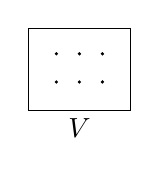
\begin{tikzpicture}[scale=0.65]
\draw (0,0) rectangle (2,1.6);
\fill (0.55,0.55) circle (0.035);
\fill (1,0.55) circle (0.035);
\fill (1.45,0.55) circle (0.035);
\fill (0.55,1.1) circle (0.035);
\fill (1,1.1) circle (0.035);
\fill (1.45,1.1) circle (0.035);
\node at (1,-0.35) {$V$};
\end{tikzpicture}
\end{adjustbox}
\begin{equation*}
\varphi(x)=\pm1,\qquad
H=-\sum_{\langle x,y\rangle}\varphi(x)\varphi(y),
\qquad \langle x,y\rangle\leftarrow\text{ближ. соседи.}
\end{equation*}
\begin{equation*}
\frac{e^{-\beta H}}{\Xi(\beta\mid V)},\qquad
\Xi(\beta\mid V)=\sum_{\varphi(V)}e^{-\beta H}.
\end{equation*}
\begin{equation*}
\begin{aligned}
\text{а)}\quad &\beta<\beta_{\mathrm{cr}}\Rightarrow
\overline{\varphi(x)\cdot\varphi(y)}\le Ce^{-\lambda\lVert x-y\rVert},
\quad\lambda=\lambda(\beta),\\
\text{б)}\quad &\beta\,\text{[}>\text{ или }\ge\text{]}\,\beta_{\mathrm{cr}}
\Rightarrow\overline{\varphi(x)\varphi(y)}\longrightarrow m^2(\beta)>0
\quad\text{(дальний порядок)},\\
\text{в)}\quad &\beta=\beta_{\mathrm{cr}}\Rightarrow
\overline{\varphi(x)\varphi(y)}\sim\frac{C}{|x-y|^{\gamma}},
\quad\gamma=\frac14\quad(d=2).
\end{aligned}
\end{equation*}
\Unclear{GELFAND-P001186}{middle-beta-sign}{В строке б): знак $>$ или $\ge$.}

В КТП возникает ситуация как с $\beta=\beta_{\mathrm{cr}}$.
Явно считается при $d=2$ своб. энергия и показатель $\gamma$.

[Разделительная черта с точкой посередине.]

\underline{Гипотеза.}
Пусть
\begin{equation*}
\varphi_L(x)=\frac{\displaystyle\sum_{y\in\Delta_L(x)}\varphi(y)}{L^\alpha}.
\end{equation*}
$\varphi$ — случ. величины (см. распр. Гиббса выше) с $\beta=\beta_{\mathrm{cr}}$.

\begin{adjustbox}{max width=\linewidth}
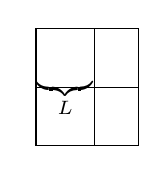
\begin{tikzpicture}[scale=0.65]
\draw (0,0) rectangle (2,2.3);
\draw (1.15,0)--(1.15,2.3);
\draw (0,1.15)--(2,1.15);
\node at (0.57,0.93) {$\underbrace{\hphantom{LLL}}_{L}$};
\end{tikzpicture}
\end{adjustbox}

Тогда совместное распределение [вставлено над строкой: случ.] величин
$\varphi_L(x)$ (при разных $x$) имеет предел и пред. распред. не зависит от модели,
с к-рой мы начали.
\begin{equation*}
x=(x_1,x_2),
\end{equation*}
\begin{equation*}
\Delta_L(x)=\{\,y=(y_1,y_2)\mid
Lx_1\le y_1<L(x_1+1),\ Lx_2\le y_2<L(x_2+1)\,\}
\end{equation*}
содержит $L^2$ точек. При разных $x$ эти квадраты не пересекаются.

Метод ренормгруппы — [зачёркнуто:
\Unclear{GELFAND-P001186}{lower-cancellation-01}{неразборчиво}]
ур-е и неподв. точки для распред.
Масштабные преобр. индуцируют преобр.
[зачёркнуто: \Unclear{GELFAND-P001186}{lower-cancellation-02}{на?}]
в мн-ве распред. вероятности.

При $d\ge4$ [зачёркнуто:
\Unclear{GELFAND-P001186}{lower-cancellation-03}{неразборчиво}]
метод тривиален — есть гауссовская неподв. точка.
Далее $d$ счит. непрер. параметром
[зачёркнуто: \Unclear{GELFAND-P001186}{lower-cancellation-04}{неразборчиво}].
$\underset{4-\varepsilon}{4}\longrightarrow3$ непрер. $\Rightarrow$ кое-что вычисл.
при $d=3$.

\underline{McPhirson}\quad
\Unclear{GELFAND-P001186}{bottom-english-title}{Perverse[последняя буква затёрта: d?] shea[исправленные буквы: f, fs?]s etc.}

(извращенные пучки)

\SourcePage{GELFAND-P001187}{unlabelled}
23/IV\quad \underline{Сем. Гельфанда.}\quad \underline{\underline{Серр.}}
О раб. [зачёркнуто: \Unclear{GELFAND-P001187}{heading-cancellation}{G\ldots?}]
\underline{Delorme и Guichardet.}

(1)\quad \underline{Лемма.}\quad $A\subset$ афф. гильбертово $H$.

$A$ огр. $\Rightarrow\exists!$ шар $\min$ радиуса, содержащий
\Unclear{GELFAND-P001187}{lemma-set-letter}{$a$ (или $A$)}.

($\min$ послед. $\Rightarrow$ центры сходятся)

(2)\quad \underline{Теорема.}
[Зачёркнут знак: \Unclear{GELFAND-P001187}{theorem-number-cancellation}{1?}]
Группа действий [вставлено: в] афф. гильб. пр-ве с
[зачёркнуто: \Unclear{GELFAND-P001187}{theorem-word-cancellation}{неразборчиво}]
огр. орбитами имеет неподв. точку.

\underline{Док-во:} центр $\min$ шара, окруж. орбиту, неподвижен.
\begin{adjustbox}{max width=\linewidth}

\begin{tikzpicture}[scale=0.7]
\fill (0,0)--(0.22,0.12)--(0,0.24)--cycle;
\end{tikzpicture}
\end{adjustbox}

\underline{Деревья.}

\underline{Св-во $(FA)$}: если $G$ действ. на дереве, то она имеет неподв. точку.

[Под $(FA)$ приписано:
\Unclear{GELFAND-P001187}{fa-gloss}{arbre; над началом слова — отдельный штрих}.]

\underline{Примеры}\quad 1) конечн.
[зачёркнуто: \Unclear{GELFAND-P001187}{examples-cancellation}{неразборчиво}]
гр.\quad 2) $SL_3(Z)$.

[Разделительная черта с точкой посередине.]

\underline{\underline{Г. Маргулис.}}
\begin{equation*}
G=G_1\times\ldots\times G_n\supset\Gamma
\qquad G_i\text{ — простые},\quad\Gamma\text{ дискретна}.
\end{equation*}
$G/\Gamma$ компактна

или $\operatorname{vol}G/\Gamma<\infty$.

Пусть не сущ. таких $G',G''$: $G=G'\times G''$
\begin{equation*}
(G'\cap\Gamma)\underset{\text{умн}}{\hphantom{\times}}(G''\cap\Gamma)
\quad\text{кон. индекса}.
\end{equation*}
\begin{equation*}
\operatorname{rank}G\ge2
\qquad(\operatorname{rank}SL(n,R)=n-1)
\end{equation*}
$\Rightarrow\Gamma$ обладает св-вом $(FA)$.

[Разделительная черта с точкой посередине.]

\SourcePage{GELFAND-P001188}{unlabelled}
3/IX--84 г.\quad \underline{\underline{Сем. Гельфанда.}}

\underline{И.М.Г.}

2 мн-зия $M_1,M_2$
\Unclear{GELFAND-P001188}{upper-overwritten-mark}{[после $M_2$ затёртый знак: запятая?]}
наз. \underline{липшицевски эквивалентными}, если $\exists$ липшиц.
гомеоморфизм (от. 2-х гладких метрик) (обр. тоже липшиц.).

\underline{Пример.}\quad пов. куба и сфера.

Гладкость не следует.

\underline{Теор. Сулливана.} На $\forall$ гладком мн-зии есть только одна липш.
структура!!

(2 гомеом. гладких мн-зия липш. эквивалентны)

\underline{Задача.} Хар. классы — интегралы от кривизн.

$g_{ik}$ должны быть $C^2$-ф-ями

(достат. 1-х?)

Как выразить классы через $g_{ik}$ без производных?
Точнее, достат. \underline{\underline{чисел}}, т.к. важно только рез. интегрирования

(ср.: обобщ. ф-и!)

\underline{Теор. Новикова} о совпад. хар. чисел гомеом. мн-зий
вытек. из теор. Сулливана.

[Разделительная черта с точкой посередине.]

\begin{equation*}
\begin{pmatrix}
\dfrac{\partial}{\partial x}&i\dfrac{\partial}{\partial y}\\
-i\dfrac{\partial}{\partial y}&\dfrac{\partial}{\partial x}
\end{pmatrix}^{2}
=
\begin{pmatrix}\Delta&0\\0&\Delta\end{pmatrix}
\end{equation*}
\Unclear{GELFAND-P001188}{matrix-01}{[Так в рукописи: оба диагональных элемента слева записаны без минуса.]}

\begin{equation*}
\begin{pmatrix}0&\operatorname{grad}\\\operatorname{div}&\operatorname{rot}\end{pmatrix}^{2}
=\Delta I\qquad(\text{в }R^4)
\end{equation*}
[Под $I$ со связующим штрихом: ед. матр.]
\Unclear{GELFAND-P001188}{matrix-02}{[Порядок grad, div, rot и обозначение $R^4$ сохранены по записи.]}

(Гамильтон)
\begin{equation*}
(d+\delta)^2=\Delta\qquad(\delta=d^*)
\end{equation*}
(на формах)

\SourcePage{GELFAND-P001189}{unlabelled}
\underline{Техника «почти всюду»} (Лебега).

Есть тело [затёрто: \Unclear{GELFAND-P001189}{upper-body-letter}{$M$ или $N$?}]
$\subset R^3$. [Ниже слева вписано: $A$.]
Объем — ? (через площади сечений)

$S(x)$ — площ. сечений.
\begin{equation*}
V=\int_a^b S(x)\,dx
\end{equation*}
$\displaystyle\int(S'(x))^2\,dx$ тоже имеет нужную размерность.

Усредним по всем напр. оси $x$.

\underline{\underline{Утв.}}
\begin{equation*}
\underset{\text{по напр.}}{\text{Средн.}}\left(\int(S'(x))^2\,dx\right)
=cV=\pi V;
\end{equation*}
$c$ не зав. от тела (как у шара).
\Unclear{GELFAND-P001189}{mean-coefficient}{[Коэффициент в рукописи: $\pi$.]}

(см. 4-й или 5-й вып. обобщ. ф-й).

\underline{Задача.} [Под заголовком: (не сделана).]
Пусть есть произвольное измеримое мн-во.
Тогда $S(x)$ измерима $(\forall x)$.
Видимо, для почти всех напр. $\exists S'(x)$.
Вопрос: в каком смысле она дифференц. и что означает ф-ла?

Это анонс Сулливана.

О препринте Гротендика \underline{«Набросок программы»}.

\underline{Перешёл:} Институт высш. исслед. $\longrightarrow$ провинц. университет.
Часть оформлена в виде рукописи 1300 стр.

\underline{Оглавление:}

1. Послание (посылка)

2. Игра Лего--Тейхмюллера и гр. Галуа $\operatorname{Gal}\overline{Q}/Q$

[Под именем: Lego--Teichmüller.]

3. Числовые поля, ассоц. с детским рисунком.

4. [Зачёркнуто: Регулярные; над строкой вставлено: Правильные]
многогранники и конечные поля.

5. \underline{Haro} об общей топ. и эвристич. размышления об умеренной топологии.

6. Дифференц. и умеренная теория a là Нэш.

7. [Зачёркнуто: \Unclear{GELFAND-P001189}{contents-07-cancellation}{Преследование?}]
В поисках полей.

8. Ответвление на
[зачёркнуто: \Unclear{GELFAND-P001189}{contents-08-cancellation}{двумерную? биградуир.?};
над строкой вставлено: 2-мерную] геометрию.

[Зачёркнута строка: (геометрия с двумя размерностями).]

9. Баланс [зачёркнуто: \Unclear{GELFAND-P001189}{contents-09-cancellation}{общего?};
над строкой: (Итог)] просветительской деятельности.

[Под «Баланс»: (Bilan).]

10. Эпилог.

\SourcePage{GELFAND-P001190}{18}
В 1970 г. прекратил публикации.

[Слева на поле зачёркнут знак:
\Unclear{GELFAND-P001190}{upper-margin-cancellation}{И?}]
Отчёт за это время.
Интуиция форм (геом.) предшествует языку.

(Топологич. и комбинаторике — перед диффер.)

\underline{Арнольд.}

\underline{Числа Каталана:}
\begin{equation*}
1,1,2,5,14,42,\ldots\qquad(\text{всего 34 определения есть})
\end{equation*}
\begin{equation*}
\frac{(2n)!}{n!(n+1)!}
\end{equation*}
Харрис ($+$ Мамфорд)

\begin{adjustbox}{max width=\linewidth}
\begin{tikzpicture}[scale=0.8]
\draw (0,0) ellipse (1.3 and 0.45);
\draw (-0.5,0.02) ellipse (0.15 and 0.1);
\draw (0.45,0.04) ellipse (0.15 and 0.1);
\node[anchor=west] at (1.65,0.05) {$g=2k$.\quad (род)};
\end{tikzpicture}
\end{adjustbox}

\begin{adjustbox}{max width=\linewidth}
\begin{tikzpicture}[scale=0.8]
\draw (0,0) circle (0.6);
\fill (-0.2,0.1) circle (0.025);
\fill (0.03,0.28) circle (0.025);
\fill (0.26,0.38) circle (0.025);
\fill (0.37,-0.03) circle (0.025);
\fill (0.2,-0.18) circle (0.025);
\fill (-0.03,-0.3) circle (0.025);
\node at (0.83,0.75) {$S^2$};
\node at (0,-0.88) {$6k$ точек};
\node[anchor=west,align=left] at (1.7,0.15) {$(k+1)$-листное накрытие\\(разветвленное)};
\draw (6.5,-0.45)--(6.65,0.7);
\draw (6.7,-0.45)--(6.85,0.7);
\node at (7.4,0.15) {$\Rightarrow$};
\node[anchor=west] at (7.95,0.15) {получ. все пов. рода $g=2k$};
\node[anchor=west,align=left] at (1.7,-1.1) {точки ветвл. — простейшие\\(квадр.)};
\end{tikzpicture}
\end{adjustbox}

$3g$ параметров (в $\mathbb{C}$).

$SL(2)$ действие $\Rightarrow3g-3$ \underline{модулей}.

Колич. раз, к-рое получ. \underline{общая поверхность} (без симметрий) —
— числа Каталана!!

[Разделительная черта с точкой посередине.]

$\Gamma\subset SU(2)$

[Под $\Gamma$ со штрихом: конечная группа.]
[Вертикальная разделительная черта.] они быв. $A_k,D_k,E_6,E_7,E_8$.

\underline{Маккей} заметил\qquad ($+$ другая связь Арнольда)

($+$ \underline{пор. монстра} связан с модулярной группой)

Рассм. гр. симметрий правильного многогр., т.е. конечную подгр.
$\Gamma\subset SU(2)$.
У неё есть конечномерные предст.
Будем $\otimes$ на другие и \underline{разлагать}. Получ. квадр. матрица —
— матр. Картана (с поправкой несущественной) аффинной системы.

\underline{Арнольд:}

\underline{случаи}; конечные гр. $\Gamma$ действ. в $\mathbb{C}^2$;
есть алгебра инвариантов, она описана.
Есть 3 завис. инварианта и одно соотнош.
[Под строкой: (т.к. пр-во 3-мерно).]
\begin{equation*}
P(x,y,z)=0
\end{equation*}
В $\mathbb{C}^3$ рассм. слой $\{P=\varepsilon\}=M_\varepsilon$,
$\dim_{\mathbb{R}}M_\varepsilon=4$.
Рассм. матр. пересеч. в 2-мерных гомологиях.
Это матрица \underline{Кокстера}. (ФА, 1972, №4)

\SourcePage{GELFAND-P001191}{unlabelled}
\underline{Группоид}: категория, в к-рой все морфизмы — изоморфизмы.

\underline{Фунд. группоид топ. пр-ва:}

точки (объекты), гомот. классы путей (морфизмы)
\begin{adjustbox}{max width=\linewidth}
\begin{tikzpicture}
\fill (0,0) circle (0.025);
\draw (0,0) .. controls (0.2,0.3) and (0.55,0.6) .. (0.95,0.57);
\fill (0.95,0.57) circle (0.025);
\end{tikzpicture}
\end{adjustbox}

\underline{Отн. пакета} точек: если не все нач. точки разрешаются.

\underline{10/IX–84 г. Сем. Гельфанда.}

\underline{М. Семенов–Тян–Шанский.}

\underline{О конференции (в Японии)!} (в окр. Киото)

\Unclear{GELFAND-P001191}{conference-morimoto}{H. / M.} Morimoto
\qquad (8 молод. японцев $+$ 8 западноевроп.)

Yosida (молодой) — интегрируемость

K. Taubs (California)

V. Kac

B. Kupershmidt

Wilson

[Справа от списка, за вертикальной чертой:]
P. [зачёркнуто: \Unclear{GELFAND-P001191}{conference-cancellation}{Van?}]
van Moerbeke. — критерий интегрируемости и неинтегрируемости,
основ. на идеях Ковалевской.

\underline{Основной итог}: открытые проблемы (будет выпущено)

\underline{О докл. P. van Moerbeke} (с [зачёркнуто: кем-то;
над строкой: Adler’ом])

Об интегрир. [зачёркнуто:
\Unclear{GELFAND-P001191}{integrability-cancellation}{реш.?}] алгебр. д.у.

По времени — мероморфные ф-и:

Разобрали левоинв. метрики на $SO(4)$

Мищенко, Фоменко $+$ ещё 2 волчка.
\begin{equation*}
\mathbb{R}^n\subset\mathbb{C}^n
\end{equation*}
\begin{equation*}
\dot z=J_{(z)}\frac{\partial H}{\partial z}=:\{z,H\}
\end{equation*}
$J(z)$ — полином, зад. скобку Пуассона, удовл. тожд. Якоби.

Скобка не обязат. невырождена.

Алгебр. [вставлено над строкой: вполне] интегрир.:

1) $\exists\ k$ полином. инвариантов $H_1,\ldots,H_k$ (Казимира)

[Справа, стрелка к «Казимира»:]
в центре скобки Пуассона (со всем коммутируют) (полиномы от $z$)

[Ниже справа, ещё одна стрелка к «Казимира»:]
центр алг. Ли, порожд. скобкой Пуассона.

2) [Затёрт знак:
\Unclear{GELFAND-P001191}{condition-02-mark}{$\exists$?}]
$m=\frac{n-k}{2}$ полином. инвар. с $\{H_i,H_j\}=0$

Тогда $\forall c_i$ (почти всех)
[зачёркнуто:
\Unclear{GELFAND-P001191}{levelset-cancellation}{$E_c\ldots$?}]
\begin{equation*}
\underbrace{\bigcap_{i=1}^{k+n}\{H_i=c_i\}}_{E_c}\cap\mathbb{R}^n
\quad\text{— лиувиллевские торы.}
\end{equation*}
\Unclear{GELFAND-P001191}{levelset-upper-bound}{Верхний предел написан $k+n$.}

(аффинный тор — либо $T^\ell$ либо $T^{\ell_1}\times\mathbb{R}^{\ell_2}$)

(теор. Лиувилля–Арнольда)

Алгебраически вполне интегрируем.

\underline{Осн. теорема.}

Алг. вполне интегр. $\Rightarrow$ 1) реш. $z_i(t)$ мероморфны по $t$;
[зачёркнуто:
\Unclear{GELFAND-P001191}{theorem-cancellation}{неразборчиво}]
\begin{equation*}
z_i(t)=\frac{z_1}{t^k}
\end{equation*}
\Unclear{GELFAND-P001191}{laurent-leading-index}{В числителе написано $z_1$; возможно $z_i$.}

[Над «разлож.» обведённая вставка: лорановское.]
[Под формулой обведено, со стрелкой влево к «разлож. реш.»: в окр. полюса.]

разлож. реш. имеют [обведённая вставка: ровно] $(n-1)$ своб. параметров

[Справа, объединено фигурной скобкой:]
$\exists\ (n-1)$-мерное сем-во лорановских решений — рядов Лорана
с полюсом в нуле (или в др. т.), удовл. системе

2)
\begin{equation*}
D_c=\left\{z_i=\frac{z_i^0}{t^p}+\ldots,\quad H_i(z(t))=c_i+\ldots\right\}
\end{equation*}
[Под $H_i(z(t))$: (не имеют полюса в нуле).]

$p\geq1$,
\Unclear{GELFAND-P001191}{pole-order-letter}{Буква порядка полюса: $p$ или $\rho$.}
$E_c\cup D_c$ — абелево мн-зие (канонич. компактификация).

$D_i$ — алгебрич. мн-зие в пр-ве $(n-1)$-пар. решений; более того, $\longrightarrow$

\Unclear{GELFAND-P001191}{bottom-divisor-index}{В последней строке индекс у $D$ похож на $i$, выше — $c$.}

\SourcePage{GELFAND-P001192}{19}
Трудность: [затёрт знак:
\Unclear{GELFAND-P001192}{top-overwritten-mark}{неразборчиво}]
постр. форм. рядов. Сходимость легче.
\begin{equation*}
\longrightarrow\bigcap_i\{H_i=c_i\}\cup D_c=\mathbb{C}^n/\Gamma
\qquad(\text{компл. тор})
\end{equation*}
\Unclear{GELFAND-P001192}{top-torus-dimension}{В показателе степени написано $n$.}

\underline{Вопрос:} как $\mathbb{C}^n/\Gamma$ связ. с якобианом
(на к-ром интегрир. ур-е).

Они не совпадают!! Но отл. факторизацией по конечн. группе.

Реш. пишется через $\theta$-ф-и.

При практич. постр. логика обращается:
начинаем с лорановских решений, зависящие от параметров.
Если $\exists$ [зачёркнуто:
\Unclear{GELFAND-P001192}{family-cancellation}{неразборчиво};
над строкой: Сем.] с $(n-1)$ своб. параметрами,
то ([зачёркнуто:
\Unclear{GELFAND-P001192}{principle-cancellation}{гипотеза?}] принцип)
есть интегрируемость.
\underline{Moerbeke} верит, что это общая теорема.

[Зачёркнуто: \Unclear{GELFAND-P001192}{example-cancellation}{Пример?}]

\underline{И. М. Г.}
\begin{equation*}
y''=f(t,y,y')
\end{equation*}
[Справа от формулы отдельный знак:
\Unclear{GELFAND-P001192}{isolated-letter}{$a$?}]

Особенности плавают.
\underline{Ур-я Пенлеве}: если \underline{особенности неподвижны}.

Неподв. особенности: для интегр. систем.

(Пенлеве рассматривал только существ. особ. точки)

Естеств. считать интегрируемыми те, когда сущ. особ. точки неподвижны.
Пенлеве — 2-й порядок.

[Над следующей строкой: Гарнье — 3-й (?)]

\underline{Задача}: дать опред. интегрируемости типа Пенлеве.
Должна быть классификация.

С. Т. Ш. \underline{Пример.}

В $\underbrace{\mathbb{R}^3}_{z_1,z_2,z_3}\oplus
\underbrace{\mathbb{R}^3}_{z_4,z_5,z_6}$ есть 2 [зачёркнуто:
\Unclear{GELFAND-P001192}{coordinates-cancellation}{неразборчиво}]
набора естеств. координат (алг. Ли $so(4)$)

[Между нижними подписями групп координат — точка с запятой.]
и $z_{ij}$ (матрицы)

[Зачёркнута строка:
\Unclear{GELFAND-P001192}{cancelled-polynomial}{$z_1z_4+z_2z_5+z_3z_6=0$?}]
\begin{equation*}
H=\frac12\sum\lambda_i z_i^2+
\sum_{i=1}^3\lambda_{i,i+3}\,z_i z_{i+3}
\end{equation*}
определяет геодезические на $SO(4)$ (в [вставлено: лево] инв. метрике);
это ур-я для прецессии [вставлено над строкой: момента];
потом надо поднять на $T^*SO(4)$.

[Под $SO(4)$ со скобкой: 6-мерный. Слева от этой подписи — две вертикальные черты.]

Интегрир. не все; часть — Манаков; Мищенко и Фоменко.

В каждом $\mathbb{R}^3$ станд. скобка (Ли–Пуасса–Березина–Кириллова)
\begin{equation*}
\{z_i,z_j\}=\varepsilon_{ijk}z_k,\qquad i,k\in1,2,3\quad\text{или }4,5,6
\end{equation*}
\begin{equation*}
\{z_i,z_{j+3}\}=0
\end{equation*}

2) $A_{ij}=\lambda_i-\lambda_j$
\begin{equation*}
(\lambda_{14}^2,\lambda_{25}^2,\lambda_{36}^2)
(A_{46}A_{32}-A_{65}A_{13})
=(A_{13}A_{46};\ A_{21}A_{54}A_{32}A_{65})\times
\end{equation*}
\Unclear{GELFAND-P001192}{bottom-product-separation}{Между $A_{54}$ и $A_{32}$ разделительный знак не виден.}

\SourcePage{GELFAND-P001193}{unlabelled}
\begin{equation*}
\times\left(
\frac{(A_{25}-A_{36})^2}{A_{32}A_{65}},\quad
\frac{(A_{36}-A_{14})^2}{A_{13}A_{46}},\quad
\frac{(A_{14}-A_{25})^2}{A_{21}A_{54}}
\right)
\end{equation*}
Здесь $D$ — из 4-х гиперэллипт. кривых (изоморфных)
с описываемым пересечением.

Идея:
\begin{equation*}
\dot L(\lambda)=[L(\lambda),M(\lambda)];
\end{equation*}
(ур. Манакова); будем счит. $\lambda$ внутренним пар.

\Unclear{GELFAND-P001193}{lax-overhead-marks}{Над $M(\lambda)$ — две горизонтальные черты и короткий вертикальный штрих.}
\begin{equation*}
\widetilde{sl}(n)=sl(n)\otimes\mathbb{C}(\lambda,\lambda^{-1})
\end{equation*}
Есть 2 скобки! 1-я трив. (Березин–Кириллов.)

2-я стр. $R$-матричным языком
\begin{equation*}
r=P_+-P_-
\end{equation*}
\begin{equation*}
\left.\operatorname{Res}(\operatorname{tr}X\cdot Y)\right|_{\lambda=0}
\end{equation*}
\begin{equation*}
\{f,g\}(L)=\bigl(\text{[зачёркнуто]}(LX)_+LY\bigr)-(XL)_+YL)
\end{equation*}
\Unclear{GELFAND-P001193}{poisson-formula}{Зачёркнутый фрагмент перед $(LX)$ не разобран; скобки и отсутствие запятых переданы как видны.}

(обобщение скобки Гельфанда–Дикого)

$X$ [зачёркнуто:
\Unclear{GELFAND-P001193}{gradient-cancellation}{$Y$?}]
$=\operatorname{grad}f$, $Y=\operatorname{grad}g$.

\underline{Для серии $SO$:} \underline{2-я} скобка не получается.

\underline{Теор. Дринфельда}: описание симплектич. слоёв в терминах
двойных смежных классов в более шир. гр. Ли.
\begin{equation*}
G\times G\longrightarrow G\qquad(\text{группа Гамильтона–Ли})
\end{equation*}
\begin{equation*}
d=g\oplus g^*\text{ — алг. Ли};\quad g,g^*\text{ — подалгебры}.
\end{equation*}
\begin{equation*}
\{\text{орбиты в }G\}=G^*\backslash D/G^*
\end{equation*}
Ф-ла, узаконяющая несохранение скобки Пуассона
\begin{equation*}
X\{f,g\}-\{Xf,g\}-\{f,Xg\}
=\langle X,[d_e\hat f,d_e\hat g]_*\rangle
\end{equation*}
Этого достат., чтобы постр. вар. гамильт. редукции.

Нет общего отобр. момента.

\underline{О Гротендике} (Сосинский).
3. \underline{Числовые поля, ассоциир. с детским рисунком.}

\SourcePage{GELFAND-P001194}{unlabelled}
\underline{8/X–84. Сем. Гельфанда.}

\underline{Бейлинсон} о раб. Атьи–Зингера

[Справа, название и строка журнала объединены фигурной линией:]

``Dirac operators coupled to vector potentials.''

\underline{Proc. Nat. Acad. Sci. USA,}

v. 81, pp. 2597–2600 (April 1984)

Построение классифицир. пр-ва калибр. группы.

Универс. опер. Дирака $\longrightarrow$ его
$\operatorname{index}{\partial\!\!\!/}\in K_0(B\mathcal{G})$

$B\mathcal{G}\simeq B(U(\infty))$
$\Rightarrow$ на $B\mathcal{G}$ есть виртуальное универс. расслоение
— оно и даёт $\operatorname{index}{\partial\!\!\!/}$.

\Unclear{GELFAND-P001194}{classifying-space-letter}{Буква в $B(U(\infty))$ похожа на $U$, но написана с острым нижним углом.}

$d\log(\det({\partial\!\!\!/}^*{\partial\!\!\!/}))$ даёт класс
$t_1\in H^1(\mathcal{G})$.

\SourcePage{GELFAND-P001195}{unlabelled}
\underline{29/X–84 г. Сем. Гельфанда.}

\underline{Семенов–Тян–Шанский} М.

\underline{Теор. Дринфельда}: класс пуасс. скобок.

$M$ — мн-зие, пусть в $C^\infty(M)$ есть скобка Пуассона
$\{\varphi,\psi\}$ — структ. алг. Ли с условием:
\begin{equation*}
(1)\qquad\{\varphi_1\varphi_2,\psi\}
=\varphi_2\{\varphi_1,\psi\}+\varphi_1\{\varphi_2,\psi\}
\end{equation*}
Тогда $M$ наз. \underline{пуассоновым}.

\underline{Это Категория} (морф. — гл. отобр., сохр. скобки)

\underline{Пуассонова группа Ли $G$}. — такая группа Ли, что

1) $G$ — пуассоново мн-зие

2)
\begin{equation*}
\begin{aligned}
G\times G&\longrightarrow G\qquad\text{— пуассоново отобр.}\\
a,b&\longmapsto ab
\end{aligned}
\end{equation*}
На $G\times G$ прямое произв. скобок
(в категории пуасс. мн-зий есть произведение)
\begin{equation*}
\{\varphi(x,y),\psi(x,y)\}
=\{\varphi(\cdot,y),\psi(\cdot,y)\}(x)
+\{\varphi(x,\cdot),\psi(x,\cdot)\}(y).
\end{equation*}
[Над строкой: или. Слева зачёркнут знак:
\Unclear{GELFAND-P001195}{product-cancelled-mark}{$\{$?}]
\begin{equation*}
\{\varphi_1,\varphi_2\}_{M_1\times M_2}
=\{\varphi_1,\varphi_2\}_{M_1}+\{\varphi_1,\varphi_2\}_{M_2}.
\end{equation*}

\underline{Примеры.}
$1^{\circ}.$ $G$ с нулевой скобкой

$2^{\circ}.$ $g$ — алгебра Ли, $g^*$ — её двойств. пр-во;
рассм. $g^*$ как аддит. гр. Ли.
Это группа Ли–Пуассона (с кан. скобкой!)

[Под «кан. скобкой»: Ли–Березина–Кириллова.]

$3^{\circ}.$ $G$ — группа Ли, причём

(i) на алгебре Ли $g$ есть инвар. скалярное произведение
[над «инвар.» вписано: невырожд.]

(ii) заданы две подалгебры $g_+,g_-\subset g$, такие, что
\begin{equation*}
g=g_+\dot{+}g_-,\quad\text{и }g_+,g_-\text{ изотропны
(отн. скалярного произв-я).}
\end{equation*}


\SourcePage{GELFAND-P001196}{unlabelled}
\underline{Упр.} (И.М.Г.) Пусть на [затушёвано:
\Incomplete{GELFAND-P001196}{header-underink}{Написанное перед $E$ закрыто густой штриховкой; чтение не восстановлено.}]
$E$ [под $E$, с выносной чертой: лин. пр-во] введ. в лин. ф-ях скобка Пуассона; тогда
на $E^*$ есть структура алгебры Ли и скобка в $E$ — из примера.

\begin{equation*}
R\in\operatorname{End}\mathfrak g:\quad R=P_+-P_-,\quad
P_\pm\text{ — проекторы на }\mathfrak g_\pm:\text{ паралл. }\mathfrak g_\mp.
\end{equation*}
\begin{equation*}
\{\varphi,\psi\}=(R(\nabla_\varphi),\nabla_\psi)
 -(R(\nabla'_\varphi),\nabla'_\psi)\tag{2}
\end{equation*}
[Выноска под $\nabla_\varphi$: левый градиент $\in\mathfrak g$;
под $\nabla'_\varphi$: прав. градиент.]

\underline{Определение градиентов.}
\begin{equation*}
(\nabla_\varphi(x),\xi)=\left(\frac{d}{dt}\right)_{t=0}\varphi(e^{t\xi}_x)
\end{equation*}
\Unclear{GELFAND-P001196}{gradient-exponential}{$x$ написан ниже $t\xi$, у правого нижнего края $e$; $e^{t\xi}_x$ или $e^{t\xi}x$.}
\begin{equation*}
(\nabla'_\varphi(x),\xi)=\left(\frac{d}{dt}\right)_{t=0}\varphi(xe^{t\xi})
\end{equation*}
\underline{Теорема 1.} (длинно доказывается). Эта скобка задаёт на $G$ структуру
пуассоновой группы Ли.

$4^{\circ}$. $G=GL(n)$
\begin{equation*}
\mathfrak g=\mathfrak n_+
 +\text{\Unclear{GELFAND-P001196}{cartan-comparison}{$\mathfrak h$ или $\mathfrak f$}}
 +\mathfrak n_-
\end{equation*}
[Выноски: под $\mathfrak n_+$ — нильп.; под средним знаком — диаг.;
под $\mathfrak n_-$ — нильп.]
\begin{equation*}
R=P_+ + AP_0\,
\text{\Unclear{GELFAND-P001196}{r-minus-overwrite}{$-$ или $+$; знак затушёван}}\,P_-,
\end{equation*}
где $A$:
\Unclear{GELFAND-P001196}{cartan-comparison}{$\mathfrak h\to\mathfrak h$ или $\mathfrak f\to\mathfrak f$; тот же двойнопетлевой знак}
— кососимм. оператор
\begin{equation*}
((A,B)=\operatorname{tr}(AB)\text{ на }gl(n))
\end{equation*}

\underline{Теорема 2} (в рамках примера $3^{\circ}$)

Симплектические листы в $G$ имеют вид
\begin{equation*}
(G_+xG_+)\cap(G_-yG_-)=M_{x,y};
\end{equation*}
(пересечения двойных смежных классов)

где $G_\pm$ — подгруппы, соотв. подалгебрам $\mathfrak g_\pm$.

Пуасс. мн-зие локально разваливается на листы-симпл. мн-зия.

\underline{Симпл. листы:} лок. пуассоново мн-зие имеет вид
\begin{adjustbox}{max width=\linewidth}

\begin{tikzpicture}[scale=0.5,baseline=0]
\draw (0,0)--(0.2,0.6);
\draw (0.12,0)--(0.32,0.6);
\draw (0.32,0)--(0.5,0.5);
\draw (0.5,0)--(0.68,0.5);
\draw (0.68,-0.08)--(0.84,0.5);
\end{tikzpicture}
\end{adjustbox}

(слоение; слои — симплектич., скобка восст. по [затушёвано:
\Incomplete{GELFAND-P001196}{symplectic-cancellation}{Слово между «по» и «симплект.» перечёркнуто густо; написанное не прочитано.}]
симплект. структ.)

На самом деле есть стратификация! (листы могут быть разных $dim$)

\underline{Опр.} Пусть $G$ — пуасс. гр. Ли, $M$ — пуасс. мн-зие; на $G\times M$ есть
пуасс. структ. Будем гов., что $G$ действ. на $M$ пуассоновым образом,
если отобр. действия $G\times M\to M$ пуассоново.

Такое действие, вообще говоря, не сохраняет скобки Пуассона на $M$.

\begin{center}
\begin{adjustbox}{max width=\linewidth}
\begin{tikzpicture}
\node (gm) at (0,0) {$G\times M$};
\node (m) at (2,0) {$M$};
\draw[->] (gm)--(m);
\draw (0.33,-0.23)--(0.33,-0.5);
\node at (0.33,-0.75) {симпл.};
\node at (5.5,0) {действ. сохр. симпл. структ.};
\node at (3.5,-0.9) {$\Downarrow$};
\node at (5.3,-1.5) {пуассоново, если на $G$ взять нулевую скобку.};
\end{tikzpicture}
\end{adjustbox}
\end{center}

\SourcePage{GELFAND-P001197}{34}
Пуассоновость действия — это равенство
\begin{equation*}
\begin{aligned}
\{\varphi,\psi\}(g\cdot x)
 &=\{\varphi(g\cdot),\psi(g\cdot)\}_M\big|_{\cdot=x}\ +\ \\
 &\quad+\{\varphi(\cdot x),\psi(\cdot x)\}_G\big|_{\cdot=g}
\end{aligned}\tag{3}
\end{equation*}
2-е слаг. измеряет несохранение скобки Пуассона.

\begin{center}
\begin{adjustbox}{max width=\linewidth}
\begin{tikzcd}
 & T^*G\arrow[dl,"\mu_{\text{п}}"']\arrow[dr,"\mu_{\text{л}}"] & \\
\mathfrak g^* & & \mathfrak g^*
\end{tikzcd}
\end{adjustbox}
\end{center}
— левое и пр. отобр. моментов;
они обр. пуассонову пару.

$M$ — симплектическое
\begin{center}
\begin{adjustbox}{max width=\linewidth}
\begin{tikzcd}
 & M\arrow[dl,"f"']\arrow[dr,"g"] & \\
X & & Y
\end{tikzcd}
\end{adjustbox}
\end{center}
— пуассоновы отобр.
Они обр. \underline{пуасс. пару}, если
[на правом поле, со стрелкой к «пуасс. пару»: \underline{или дуальную пару}]
\begin{equation*}
\{f^*C^\infty(X),g^*C^\infty(Y)\}=0
\end{equation*}
Наз. пару \underline{полной}, если одна из алгебр $f^*C^\infty(X)$, $g^*C^\infty(Y)$ является
централизатором другой:
\begin{equation*}
f^*C^\infty(X)=(g^*C^\infty(Y))^\perp
\end{equation*}
\Unclear{GELFAND-P001197}{centralizer-perpendicular}{В показателе после скобки написан $\perp$; значение этого обозначения централизатора не пояснено.}

\underline{Теорема 3} (в лок. форме т-мы). В этой ситуации
[зачёркнуто: $g(f^{-1}(x))$] и
$f(g^{-1}($\Unclear{GELFAND-P001197}{theorem-three-fibre}{$y$ или $x$; буква переправлена}$))$
— симплектический лист!

(и локально все симпл. листы так получаются)

Хотим применить это к док-ву теор. Дринфельда.
\begin{center}
\begin{adjustbox}{max width=\linewidth}
\begin{tikzcd}
 & M\arrow[dl]\arrow[dr] & \\
G & & X
\end{tikzcd}
\end{adjustbox}
\end{center}
[Под $G$, с выносной чертой: задано.]

Для произв. пуассоновой гр. Ли строится дубль $D$ (группа удвоенной $dim$)
\begin{center}
\begin{adjustbox}{max width=\linewidth}
\begin{tikzcd}
 & D\arrow[dl]\arrow[dr] & \\
G & & G
\end{tikzcd}
\end{adjustbox}
\end{center}
$G=\mathfrak g^*\Rightarrow$ получ. конструкция
Ли–Кириллова–Костанта
\begin{equation*}
\mathfrak d=\mathfrak g\oplus\mathfrak g^*,\quad
(\mathfrak g^*\text{ — тоже алгебра Ли, т.к. есть пуасс. структура на }G)
\end{equation*}
$D$ — гр. Ли алгебры $\mathfrak d$

На $\mathfrak d$ есть естеств. скал. произвед.:
\begin{equation*}
\langle(X,F),(X',F')\rangle=F(X')+F'(X)
\end{equation*}
Это сводит к примеру $3^{\circ}$: на дубле появл. структ. гр. Ли–Пуассона.

\SourcePage{GELFAND-P001198}{unlabelled}
На $G$ есть далее 2 скобки Пуассона:
\begin{equation*}
\{\varphi,\psi\}_\pm(x)
 =(R(\nabla_\varphi(x)),\nabla_\varphi(x))
 \pm(R(\nabla'_\varphi(x)),\nabla'_\varphi(x))
\end{equation*}
\Unclear{GELFAND-P001198}{bracket-subindices}{В обоих слагаемых оба нижних индекса имеют вид $\varphi$, при $\{\varphi,\psi\}$ слева.}

На $D$ надо взять скобку со знаком $+$.

$\pm$ связ. со св-вами однородности скобки Склянина.

\underline{Теорема 4.} 1) Пусть $G$ — гр. Ли–Пуассона, $D$ — её дубль. Тогда канонические
проекции $D\to D/G^*$ и $D\to G\backslash D$ образуют полную
дуальную пуассонову пару.
\Unclear{GELFAND-P001198}{theorem-four-quotient}{В тексте $G\backslash D$ без звёздочки, в рисунке $G^*\backslash D$.}

\SourceFigure{GELFAND-P001198}{diagram-left-overwrite}{Сверху $D^{(+)}$; две стрелки вниз: влево к $D/G^*$, вправо к $G^*\backslash D$. Между $D$ и $G^*$ слева густо переправленный косой знак, похожий на $/$; его нижний слой не восстановлен.}

2) $G\subset D/G^*$ и структ. индуцируется.
[Под $G$, с выносной чертой: \underline{откр. клетки}.]

[Разделительная линия: два штриха и точка.]

$H\subset G$ [выноска от $H$: подгр.]
\begin{equation*}
C^\infty(M)^H\subset C^\infty(M)
\end{equation*}
\underline{Теор. 5.}
\begin{equation*}
C^\infty(M)^H\text{ — подалгебра Ли}\ \Leftrightarrow
\text{\Unclear{GELFAND-P001198}{annihilator-symbol}{$\mathfrak h^\perp$ или $\mathfrak f^\perp$}}
\subset\mathfrak g^*\text{ — подалгебра Ли}
\end{equation*}
[От знака со степенью $\perp$ проведена выноска вниз к зачёркнутому:
\Incomplete{GELFAND-P001198}{annihilator-cancel}{Написанная под формулой помета густо перечёркнута; видны лишь отдельные начальные штрихи, полного чтения нет.}]

\underline{Д-во.}
\begin{equation*}
X\{\varphi,\psi\}-\{X\varphi,\psi\}-\{\varphi,X\psi\}
 =\langle[d_e\varphi(g\cdot x),d_e\psi(g\cdot x)]_*,X\rangle
\end{equation*}

[Разделительная линия: два штриха и точка.]

Пусть $G$ — группа Пуассона–Ли у примера $3^{\circ}$.

$M\subset G$ — симплектич. лист
\begin{equation*}
T\in M,\quad D:\underline{G}\times M\to M
\end{equation*}
\begin{equation*}
D(g,T)=(TgT)_+^{-1}T
\end{equation*}
\Unclear{GELFAND-P001198}{d-action}{Внутри скобок $TgT$; $-1$ виден только снаружи, над индексом $+$.}

(использ. лок. разложение $x=x_+x_-$, $x_\pm\in G_\pm$)

\underline{Теор. 6.} Это действие \underline{пуассоново}

Квантовая группа — объект, при классич. пределе перех. в [зачёркнуто:
\Incomplete{GELFAND-P001198}{quantum-cancel-full}{Слово после «в» и перед «групп.» закрыто перечёркиванием; написанное не прочитано.}]
групп.
[Вписано снизу под «перех.»: алгебру.]

(\underline{Дринфельд}:
группа и когруппа; обе опер. — ряды по $h$)

\underline{Алг. Склянина:} ФА, 17:4



\end{document}
